\documentclass{beamer}

\usepackage[czech]{babel}
\usepackage[utf8]{inputenc}
\usepackage[T1]{fontenc}
\usepackage{cite}
\usepackage{algorithmic}
\usepackage{csquotes}
\usepackage{algorithm}
\usepackage{graphicx}
\usepackage{xcolor, picture}


\usetheme{Madrid}

\setbeamertemplate{footline}{
  \begin{beamercolorbox}[wd=\paperwidth, sep=1ex]{footlinecolor}
    \hspace*{2ex}
    \insertframenumber/\inserttotalframenumber \hfill
    \inserttitle \hfill
    \insertauthor \hfill
    \insertdate
    \hspace*{2ex}
  \end{beamercolorbox}
}
\setbeamercolor{footlinecolor}{fg=white,bg=blue!90!black}
\setbeamertemplate{navigation symbols}{}


\title{Typografie a~publikování\,--\,5.projekt\\
Zásobník}
\author{Martin Kováčik}
%\institute{\textsc{FIT\,--\,VUT}}
\date{\today}

\begin{document}

\begin{frame}
  \titlepage
  \begin{figure}[h]
    \centering
    \scalebox{0.1}{
\includegraphics{FIT_LOGO.png}}
\end{figure}
\end{frame}

\begin{frame}{Obsah}
  \tableofcontents
\end{frame}

\section{Proč rozumět zásobníku}
\begin{frame}{Proč se rozumět zásobníku}

  \begin{itemize}
      \item \textbf{Základní stavební kámen:} Znalost zásobníku je klíčová pro pochopení složitějších konceptů v~informatice.
        \item \textbf{Praktické využití:} Znát zásobník znamená mít na dosah ruky efektivní řešení pro mnoho problémů
            \item \textbf{Rozvoj dovedností:} Učení se zásobníkům podněcuje kreativitu, logické myšlení a~práce s~ním napomáhá k hledání elegantních řešení

\end{itemize}
\end{frame}

\section{Úvod}
\begin{frame}{Úvod}
  \begin{itemize}
      \item Jednoduchá datová struktura s~proměnným počtem zařazených prvků. 
        \item Spojový seznam fungující na principu LIFO (Last-In-First-Out) nebo~také pushdown store.
        \item Základní sada operací zásobníku obsahuje instrukce:\cite{wikisofia-datove-struktury}
        \begin{itemize}
            \item vložit (Push)
            \item vybrat (Pop)
            \item test prázdnoty (Empty)
        \end{itemize}
  \end{itemize}
\end{frame}

\section{Princip zásobníku}
\begin{frame}{Ukázka zásobníku}
    
\begin{figure}[h]
    \centering
    \scalebox{0.3}{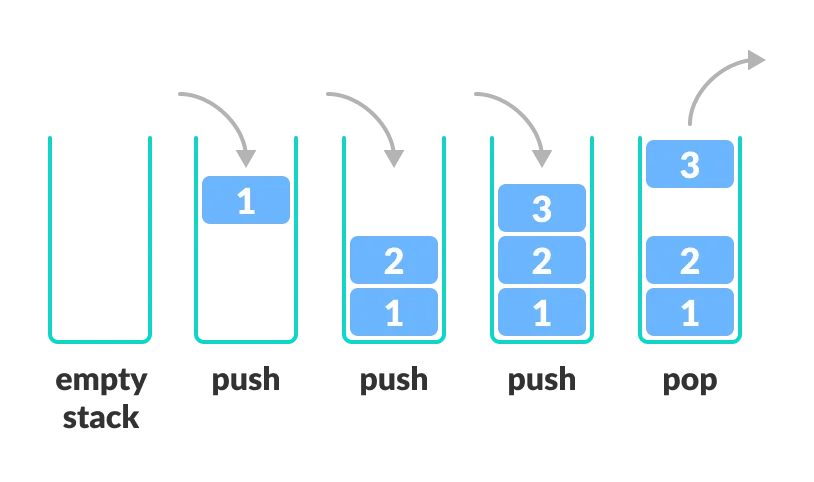
\includegraphics{Stack.png}}
    \caption{Obrázek: Ilustrace zásobníku. Získáno z~\url{https://cdn.programiz.com/sites/tutorial2program/files/stack.png}.}
\end{figure}
\end{frame}

\section{Historie}
\begin{frame}{Historie}
  \begin{itemize}
  \item Koncept zásobníků neformálně zavedl Alan Turing\cite{duplessis2023}
    \item Zásobník byl poprvé použit v~50.~letech 20.~století pro práci s~podprogramy v~rámci programování      
        \item Teprve v~roce 1957 se pro tuto konkrétní datovou strukturu užil termín stack (zásobník).
  \end{itemize}
  \vspace{3.0em}
    \begin{block}
    
    v~průběhu let se zásobník stal důležitou součástí počítačové vědy a~je využíván v~široké škále oblastí od algoritmů a~datových struktur po programování.
    \end{block}
\end{frame}

\section{Axiomy pro operace se zásobníkem}
\begin{frame}{Axiomy pro operace se zásobníkem}

  \begin{algorithm}[H]
\caption{Axiomy pro operace se zásobníkem}
\begin{algorithmic}[1]
    \STATE \textbf{Axiom 1:} \textbf{isempty}(\textbf{create}());
    \STATE \textbf{Axiom 2:} $\neg$\textbf{isempty}(\textbf{push}($x$, $S$));
    \STATE \textbf{Axiom 3:} \textbf{pop}(\textbf{push}($x$, $S$)) $=$ $S$;
    \STATE \textbf{Axiom 4:} \textbf{top}(\textbf{push}($x$, $S$)) $=$ $x$;
    \STATE \textbf{Axiom 5:} $\neg$\textbf{isempty}($S$) $\Rightarrow$ (\textbf{push}(\textbf{top}($S$), \textbf{pop}($S$)) $=$ $S$);
\end{algorithmic}
\end{algorithm}

\begin{itemize}
\item[*] \emph{Henriksson ve svém článku "A Brief History of the Stack" poskytuje přehled vývoje zásobníku v~informatice. Tyto axiomy byly převzaty z~tohoto zdroje.}\cite{henriksson_stack_history}
\end{itemize}
\end{frame}


\section{Závěr}
\begin{frame}{Závěr}
  \begin{block}
  
  Pochopení a~efektivní používání zásobníků je nezbytností pro mnoho oblastí programování a~informatiky.\cite{shukla_stack}
  \end{block}
  
  \begin{itemize}
      \item Zasobník je a~ještě nějakou dobu bude součást programování
      \item Bez zásobníku je náročné tvořit složitější alogoritmy
      \item Se zásobníkem se setkáme v~každodenní praxi a~nevyhneme se mu 
      \item Pro každého programátora je znalost zásobníku klíčová
  \end{itemize}
\end{frame}




\section{Zdroje}
\begin{frame}{Použité zdroje}
	\bibliographystyle{czechiso}
	\renewcommand{\refname}{Použité zdroje:}
	\bibliography{proj5}
\end{frame}


\end{document}